In den Versuchen hatten die verwendeten Bauteile folgende Werte, welche im folgenden
für die Auswertung verwendet werden:
\begin{itemize}
    \item Widerstand 1: $R_1 = 48,1 \pm 0,1 \mathrm{ohm}$
    \item Widerstand 2: $R_2 =509,5 \pm 0,5 \mathrm{ohm}$
    \item Kondensator: $C = 2,089 \pm 0,006 \mathrm{nF}$
    \item Spule: $L = 10,11 \pm 0,03 \mathrm{mH}$
\end{itemize}
\subsection{Zeitabhängikeit der Amplitude}
Um die Zeitabhängigkeit der Amplitude zu bestimmen, wurde die Spannung $U$ in Abhängigkeit der Zeit $t$ gemessen. 
Die Messwerte sind in Tabelle 1 dargestellt. 
\begin{table}[H]
    \centering
    \begin{tblr}{c c c}
    \toprule
    $Messung$ & $Spannung$  U in V & Zeit $\delta t$ in $\mu$s \\
    \midrule
    $T_0$ & 0.62 & 20 \\
    $T_1$ & 0.57 & 30 \\
    $T_2$ & 0.53 & 50 \\
    $T_3$ & 0.48 & 60 \\
    $T_4$ & 0.43 & 75 \\
    $T_5$ & 0.40 & 90 \\
    $T_6$ & 0.36 & 105 \\
    $T_7$ & 0.33 & 120 \\
    $T_8$ & 0.30 & 135 \\
    $T_9$ & 0.27 & 150 \\
    $T_{10}$ & 0.25 & 165 \\
    $T_{11}$ & 0.23 & 180 \\
    $T_{12}$ & 0.21 & 195 \\
    $T_{13}$ & 0.20 & 210 \\
    $T_{14}$ & 0.18 & 225 \\
    $T_{15}$ & 0.16 & 240 \\
    \bottomrule 
    \end{tblr}
    \caption{Messreihe zur Zeitabhängigkeit der Amplitude}
\end{table}
\noindent
Die Zeit wurde in delta t gemessen, da die Zeit zwischen den einzelnen Peaks der Spannung gemessen wurde.
Die Spannung wurde über die Peak-to-Peak Methode bestimmt, und dann durch zwei geteilt, um die Amplitude zu erhalten.
Aus den Messwerten wurde ein Fit der Form $U(t) = U_0 \cdot e^{-\frac{R}{2L}t}$ durchgeführt, um den Widerstand R zu bestimmen.
Die Messwerte und der Fit sind in Abbildung 3 dargestellt.
\begin{figure}[H]
    \centering
    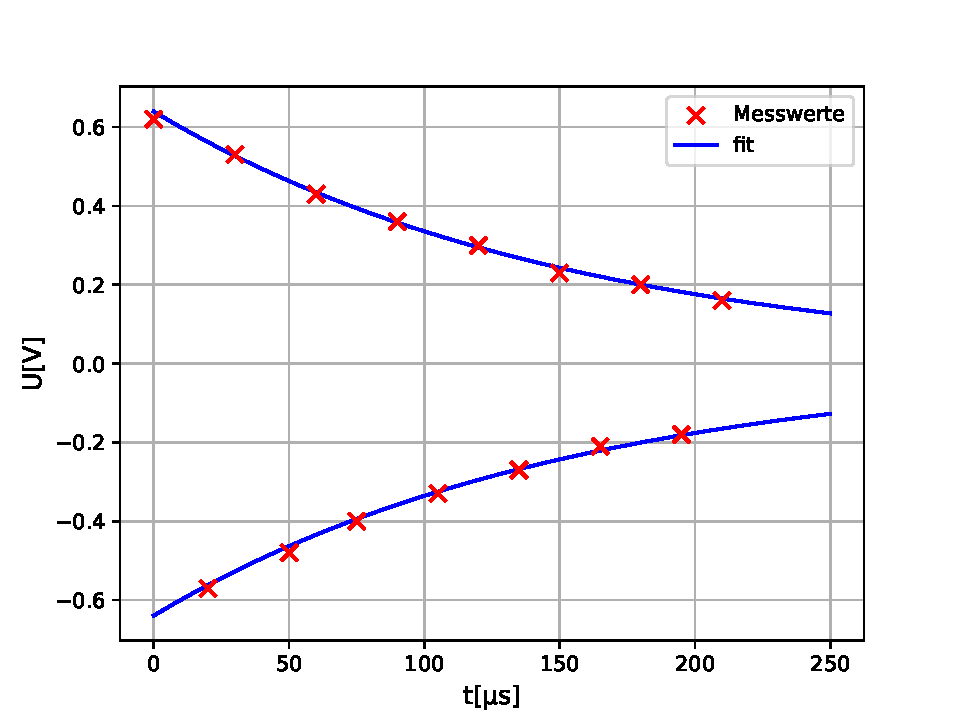
\includegraphics[width=0.8\textwidth]{v354/Exp_Abfall.pdf}
    \caption{Messwerte und Fit der Zeitabhängigkeit der Amplitude}
    \label{fig:exp_abfall}
\end{figure}
\noindent
Der Fit wurde in der Form $f(x) = a \cdot e^{b \cdot x}$ durchgeführt, wobei $a$ und $b$ die Fitparameter sind.
Aus dem Fit wurde der Wiederstand R bestimmt(\ref{fig:exp_abfall}). Der Fit ergab einen Wert von $b = -6449.56 \pm 102,52 \mathrm{Hz}$. Daraus ergibt sich ein Widerstand von:
\begin{equation}
    R_{\text{Fit}} = 2 \cdot L \cdot b \cdot (-1) = 130,39 \mathrm{\Omega}
\end{equation}
Die Ungenauigkeit des Widerstands wurde über die Fehlerfortpflanzung bestimmt. Die Fehlerfortpflanzung ergibt sich aus der Formel:
\begin{equation}
    \Delta R = \sqrt{(\frac{\partial R}{\partial L} \cdot \Delta L)^2 + (\frac{\partial R}{\partial b} \cdot \Delta b)^2}
\end{equation}
Damit ergibt sich eine folgende Ungenauigkeit des Widerstands:
\begin{gather}
    \Delta R = 2 \cdot \sqrt{(b \cdot \Delta L)^2 + (L \cdot \Delta b)^2} = 2 \\
    \sqrt{(6449,56 \cdot 0,03)^2 +(10,11 \cdot 102,52)^2} = 2,08 \mathrm{\Omega}\\
    R_{\text{Fit}} = 130,39 \pm 2,08 \mathrm{\Omega}
\end{gather}

\subsection{Aperiodischer Grenzfall}
Der Widerstand, der für den Aperiodischen Grenzfall benötigt wird, lässt sich mit folgender Formel bestimmen:
\begin{equation}
    R_{\text{Theorie}} = 2 \cdot \sqrt{\frac{L}{C}}
\end{equation}
Damit ergibt sich ein Widerstand von:
\begin{equation}
    R_{\text{Theorie}} = 2 \cdot \sqrt{\frac{10,11 \cdot 10^{-3}}{2,089 \cdot 10^{-6}}} = 4399,83 \mathrm{\Omega}
\end{equation}
Der Aperiodische Grenzfall wurde über ein vestellbaren Widerstand bestimmt, der zwischen 1 und 10000 Ohm einstellbar ist.
 Der Widerstand wurde zunächst auf seinen Maximalwert eingestellt und dann langsam verringert, bis der Aperiodische Grenzfall eintrat. 
 Danach wurde der Widerstand auf seinen Minimalwert eingestellt und langsam erhöht, bis der Aperiodische Grenzfall eintrat. 
Der Aperiodische Grenzfall trat beim ersten Versuch bei einem Widerstand von $R_{\text{exp1}} \approx 3200 \mathrm{\Omega}$ ein.
Beim Zweiten Versuch trat der Aperiodische Grenzfall bei einem Widerstand von $R_{\text{exp2}} \approx 3160 \mathrm{\Omega}$ ein.
\subsection{Frequenzabhängigkeit der Kondensatorspannung und Phase}
Um die Frequenzabhängigkeit der Kondensatorspannung und der Phase zu bestimmen, 
wurde die Spannung des Kondensators $U_C$ und die Spannung des Erregers $U_{Err}$ in Abhängigkeit der Frequenz $f$ gemessen, siehe Tabelle 2.
\begin{table}[H]
    \centering
    \caption{Frequenzabhängigkeit der Kondensatorspannung und Phase}
    \begin{tblr}{c c c c}
    \toprule
    Frequenz in $kHz$ & $U_C$ in V & $U_{Err}$ in V & Verschiebung \\
    \midrule
    10.0 & 1.05 & 0.8 & 0.00 \\
    20.0 & 1.25 & 0.8 & 0.00 \\
    27.9 & 2.05 & 0.8 & 0.3 \\
    28.4 & 2.15 & 0.8 & 0.3 \\
    28.9 & 2.25 & 0.8 & 0.3 \\
    29.4 & 2.35 & 0.8 & 0.4 \\
    29.9 & 2.45 & 0.8 & 0.4 \\
    30.4 & 2.55 & 0.8 & 0.5 \\
    30.9 & 2.65 & 0.8 & 0.5 \\
    31.4 & 2.75 & 0.8 & 0.6 \\
    31.9 & 2.85 & 0.8 & 0.6 \\
    32.4 & 2.85 & 0.8 & 0.6 \\
    32.9 & 2.85 & 0.8 & 0.7 \\
    33.4 & 2.85 & 0.8 & 0.7 \\
    33.9 & 2.80 & 0.8 & 0.8\\
    34.4 & 2.70 & 0.8 & 0.8 \\
    34.9 & 2.55 & 0.8 & 0.8 \\
    35.4 & 2.45 & 0.8 & 0.9 \\
    35.9 & 2.35 & 0.8 & 0.9 \\
    36.4 & 2.15 & 0.8 & 1 \\
    36.9 & 2.10 & 0.8 & 1\\
    37.4 & 1.95 & 0.8 & 1 \\
    37.9 & 1.85 & 0.8 & 1 \\
    50.0 & 0.65 & 0.8 & 0.9 \\
    \bottomrule
    \end{tblr}
\end{table}
Damit ergibt sich die Resonanzfrequnez aus der Messung bei $f_{\text{res}} = 32,9 \mathrm{kHz}$.
Die Theoriewerte für die Resonanzfrequenz und die Güte des Schwingkreises lassen sich über folgende Formeln bestimmen:
\begin{equation}
    f_{\text{res, Theorie}} = \frac{1}{2 \pi \sqrt{L \cdot C}} = 34,7 \mathrm{kHz}
\end{equation}
Und die Kondensatorspannung in abhängigkeit der Frequenz lässt sich über folgende Formel bestimmen:
\begin{equation}
    U_C(f) = \frac{U_0}{\sqrt{(1 - (2 \pi f)^2 L C)^2 + (2 \pi f R C)^2}}
\end{equation}
Den Plot der Kondensatorspannung und der Phase in Abhängigkeit der Frequenz ist in Abbildung 4 dargestellt.
\begin{figure}[H]
    \centering
    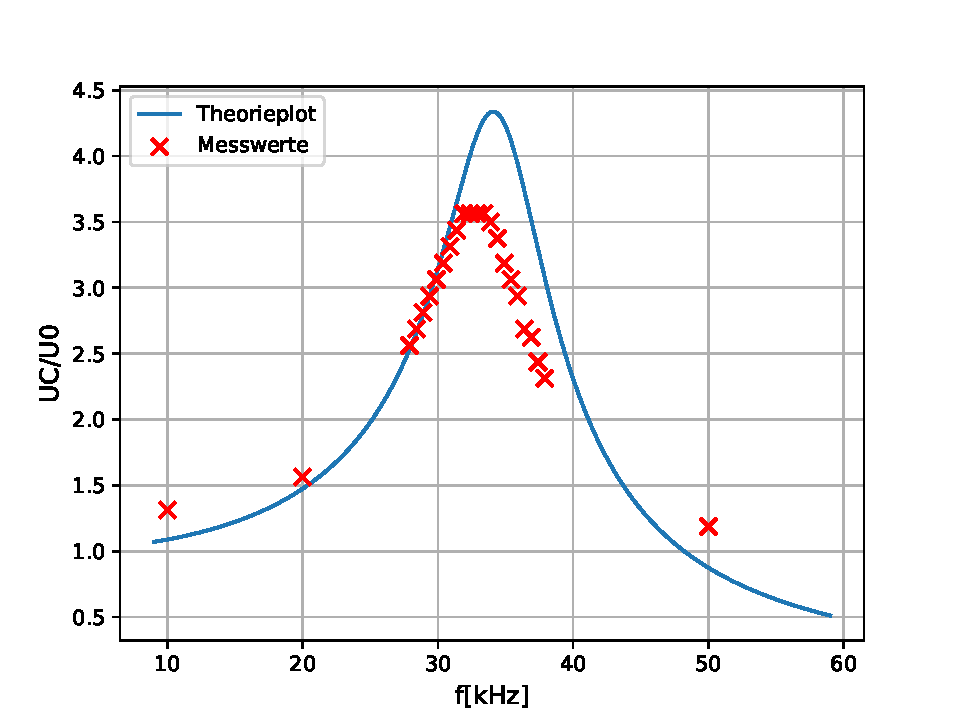
\includegraphics[width=0.8\textwidth]{v354/Spannungsamplitude.pdf}
    \caption{Kondensatorspannung in Abhängigkeit der Frequenz}
    \label{fig:amp}
\end{figure}
Die Phasenverschiebung lässt sich über folgende Formel bestimmen:
\begin{equation}
    \phi(f) = \arctan{\Bigl(\frac{-2 \pi f R C}{1 - (2 \pi f)^2 L C}\Bigr)}
\end{equation}
Die aus den Messwerten bestimmte Phasenverschiebung ist in abhängigkeit der Frequenz in Abbildung 5 dargestellt.
\begin{figure}[H]
    \centering
    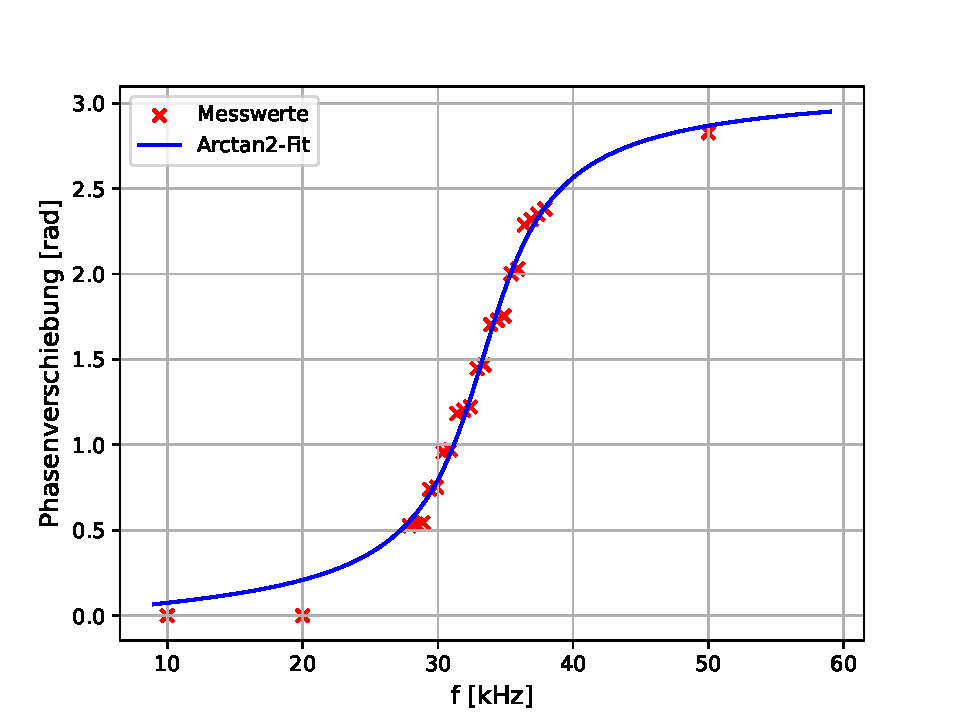
\includegraphics[width=0.8\textwidth]{v354/Arctan2.pdf}
    \caption{Phasenverschiebung in Abhängigkeit der Frequenz}
    \label{fig:phase}
\end{figure}
\subsection{Güte des Schwingkreises}

4 Wege Güte zu errechnen
Theoriewert Resonanzbreite aus amp.plot%1/sqrt(2)
Hochpunkt aus amp.plot
resonanzbreite aus phasen.plot (45,90,135 grad)